% Verification on rough terrain (tests/soilzone/test_rough_terrain.py, rough_models.py, rough_ext.py, rough_cases/).
\section{Verification on rough terrain}\label{sec:vrough}
The tests of Section~\ref{sec:vsoilzone} use planar hillslopes. Real ground is irregular: slopes change within a cell,
the land holds pits, closed depressions, cliffs and ridges, the DEM is finer or coarser than the grid and may end inside
it, and the MODFLOW layers slope, thin out and pinch against bedrock. The rough-terrain suite
(\cmd{tests/soilzone/test\_rough\_terrain.py}) draws such cases at random from a seed, runs each with every
unsaturated-zone method and checks every run against rules that hold whatever the ground looks like. A seed always gives
the same case, so every failure can be replayed (\cmd{--case}).

\subsection{What the cases vary}
Every fourth seed couples an existing MODFLOW~6 model written by the suite (\cmd{rough\_ext.py},
Section~\ref{sec:vexisting}); the others let Raven build the model (\cmd{rough\_models.py},
Section~\ref{ch:layers}). Table~\ref{tab:vroughvary} lists the ranges.
\begin{table}[!htbp]\centering
\caption{What the rough-terrain cases vary (\cmd{rough\_models.gen\_spec}; existing models: \cmd{rough\_ext.ext\_spec}).}\label{tab:vroughvary}\small
\begin{tabular}{P{0.2\linewidth}P{0.74\linewidth}}\toprule\hdr
Item & Range\\\midrule
ground & a plane sloping 0--30\,\% in any direction plus roughness: spectral noise, bumps, pits, closed depressions, cliffs (steps a few metres wide, or sharper than the DEM) and ridges; relief within a cell from 0.05 to 6 times the soil-zone thickness $D$\\
DEM & resolution 0.08--1.6 cells; NODATA holes; a DEM that ends inside the grid (cells partly without land samples)\\
grid and HRUs & cells of 25--150~m, 4--9 by 3--6 cells; a tiling of HRUs cut at random positions (on and off cell edges, one-cell HRUs); domain edges on or inside cells; \cmd{:MinCellCoverage} 0.1--0.5\\
soil & two soil profiles by position, two layers, $D$ 0.3--3~m; Campbell retention for the capillary rise; \cmd{PERC\_CONSTANT} or \cmd{PERC\_GAWSER\_CONSTRAIN}\\
aquifer (generated) & two aquifer profiles by position, 1--3 layers of 2--3 classes ($K_h$ 0.05--30~m/d, $K_v$ down to $10^{-2.5}K_h$, $S_y$ 0.02--0.3, retention for the columns); thin layers (0.2--0.8~m); sloping bedrock raster (or \cmd{DEFAULT\_BEDROCK\_DEPTH}), so layers slope, pinch out, are clipped at bedrock and become pass-through cells; bedrock at least $\max D+1.0123$~m below the land, except in outcrop cases (bedrock above the soil-zone base under a whole HRU)\\
aquifer (existing) & DIS or DISV (irregular quadrilaterals); top = mean land $-D$, moved up or down by up to $D$; 1--3 layers whose thicknesses tilt across the model, pass-through cells (\cmd{IDOMAIN}~$-1$) where a layer thins below 0.5~m, inactive columns and columns with an inactive first layer (\cmd{IDOMAIN}~0); a confined bottom layer in some models; \cmd{NEWTON} in most models, a few without it\\
water & \cmd{:SoilZoneSubgrid} 1, 3, 5, 9; \cmd{SEEPAGE\_SMOOTHING\_DEPTH} 0.02--0.5~m; 40--90 daily steps; mean rain 8--45~mm/d on 10--40 wet days (daily 2.4--77~mm/d) between dry spells; soil evaporation 0--4~mm/d; start deep (3--15~m), shallow (0.2--2~m) or at the land; a specified head along the low edge; \cmd{:SoilZoneCapillaryRise} on, off or default; \cmd{:SoilZoneExchangeTiming} \cmd{LAGGED} or \cmd{AFTER}\\
\bottomrule
\end{tabular}
\end{table}

\subsection{What every run is checked for}
\begin{description}
\item[Run] The run completes, or stops with a justified message (below).
\item[Finite] No NaN or Inf in any output table, no non-finite head, no \cmd{HDRY} head in an active cell under \cmd{NEWTON}.
\item[Balances] The identities of Section~\ref{sec:audit} close within the standard limits (recharge $5\times10^{-9}$,
soil zone and unsaturated zone $10^{-8}$, MODFLOW $10^{-5}$ of the recharge, Raven $10^{-5}$~mm), and no soil-zone
shortfall is booked on a step whose interface converged.
\item[Layers] For generated models, \cmd{TOP}, \cmd{BOTM} and \cmd{IDOMAIN} as MODFLOW read them equal an independent
construction from the DEM, the bedrock raster and the profiles (Section~\ref{ch:layers}) within $10^{-6}$~m.
\item[Bases] The soil-zone base of every HRU equals the overlap-weighted land surface of its cells less $D$ (existing
models: the top of the top active cell).
\item[Saturated fraction] With \cmd{:SoilZoneVadose NONE}, the saturated fraction of every HRU equals an independent
closure --- the cell's DEM samples less $D$, none below 1~mm above the top cell's bottom, smoothed over $d_s$ --- at a head
between the top cells' heads at the start and the end of the step, on every converged step, within 0.02. With a column
method the difference is reported only: the fraction reported for a link whose column carries the step is the
connection's, not the one that rejected the recharge.
\item[Physics] $0\le F\le1$; soil water within $[0,$ capacity$]$; rejected recharge and overflow $\ge0$; with
\cmd{NONE} the rejected recharge is at most the HRU's recharge, positive only where $F>0$, and $F$ times the recharge on
HRUs over one cell; with a column method the rejected recharge of a step is at most its recharge plus the columns'
storage at its start.
\item[Heads] With a column method, no water table more than 5~m above the highest land sample of its cell, unless the
\cmd{NONE} run of the same case lifts it to within 1~m of that height.
\item[Convergence] Steps on which MODFLOW or the interface did not converge are counted; more than 5\,\% fails the case.
\end{description}
A run whose failures are all known ones is reported as a known failure (XFAIL): the suite keeps one known pattern, an
interface left unconverged where the land lies below the top cell's bottom, and no open case. A shortfall is never a known
failure, and a regression case's own checks are added before this is decided: any other failure makes the run fail.

\paragraph{Justified stops.} A run may stop without failing in three situations: an outcrop case (\emph{HRU \dots\ does
not overlap any active groundwater cell}); an existing model without \cmd{NEWTON} (\emph{:SoilZone PHYSICAL needs an
existing model that uses the Newton-Raphson formulation}); and a diverged solve (\emph{heads are not finite}, or a head
far outside the model on an unconverged step) that MODFLOW~6 repeats on its own. For the last, the suite runs the case's
MODFLOW model through the library without Raven's packages, with a drain at the top of every column as the only outlet
and no recharge, for the run's duration; the stop is justified only if those heads become non-finite or move by more
than $10^6$~m within the outer iterations. A column held 1~mm above its bottom (Section~\ref{sec:drained}) is reported,
not a failure.

\paragraph{Regression cases.} Twenty cases run first (R1--R20): R1 is a flat hillslope (the configuration of P3
without columns), on which an interface that passed as converged with the saturated fraction of an earlier iterate
rejected 15\,\% of the recharge where the closure at the step's heads allows at most 5\,\%; R2--R20 are stored cases
(\cmd{rough\_cases/*.json}, each with its spec and the meta data the checks use) for the problems the suite found. Each has
its own checks besides the above: R6, R11--R13 and R19 must complete (no stop at all), and R20 (stored existing model e43,
\cmd{LAG}) must hold the saturated fraction to the closure within 0.004 with any method: its land lies in
places within the 1~mm band above the top cell's bottom, where no sub-grid base may lie. \cmd{--case} applies these checks
too when it replays a stored case.

\subsection{Results}
Table~\ref{tab:vroughres} summarizes the suite's 400 default seeds run with each of the four methods
(\cmd{--methods NONE,RICHARDS,KINEMATIC,LAG}, 1\,620 runs with the regression cases; the script's default runs
\cmd{NONE} and \cmd{RICHARDS} only). No run failed and none was a known failure. Every run that completed (1\,567 of
1\,620) closed all balances within the limits above (largest values: recharge identity $4.5\times10^{-10}$, soil-zone
identity $9.9\times10^{-10}$, unsaturated-zone identity $4.6\times10^{-10}$, MODFLOW $7.7\times10^{-6}$ of the recharge,
Raven $10^{-11}$~mm; largest shortfall $4\times10^{-14}$). The independent geometry agreed everywhere: layers to
$5\times10^{-8}$~m, bases to $5\times10^{-8}$~m. On converged steps the saturated fraction agreed with the closure to
0.0022 with \cmd{NONE} (limit 0.02); with a column method it is reported (largest difference 0.0027 with \cmd{RICHARDS}
and \cmd{LAG}, 0.0020 with \cmd{KINEMATIC}).
\begin{table}[!htbp]\centering
\caption{Rough-terrain suite, default seeds and regression cases, one depth class.
Run times depend on the machine and its load (the rerun shared two cores with another test suite).}\label{tab:vroughres}\small
\begin{tabular}{P{0.36\linewidth}P{0.13\linewidth}P{0.13\linewidth}P{0.13\linewidth}P{0.13\linewidth}}\toprule\hdr
 & \cmd{NONE} & \cmd{RICHARDS} & \cmd{KINEMATIC} & \cmd{LAG}\\\midrule
runs & 407 & 408 & 401 & 404\\
completed / justified stops & 393 / 14 & 395 / 13 & 388 / 13 & 391 / 13\\
known failures / failures & 0 / 0 & 0 / 0 & 0 / 0 & 0 / 0\\
time steps of completed runs & 25\,753 & 25\,809 & 25\,350 & 25\,528\\
steps with the interface unconverged & 0 & 0 & 0 & 0\\
steps with MODFLOW unconverged & 0 & 0 & 0 & 0\\
runs with the water table $>5$~m above the land; largest & 44; 94.2~m & 43; 94.2~m & 40; 94.2~m & 42; 94.2~m\\
MODFLOW outer iterations per step (mean) & 6.34 & 5.83 & 5.70 & 7.20\\
mean run time [s] & 0.16 & 0.22 & 0.18 & 0.19\\\bottomrule
\end{tabular}
\end{table}
The justified stops are the outcrop cases (g14, g33, g58, g61, g162, g223, g266), the existing models without
\cmd{NEWTON} (e36, e96, e200, e256, e316, e356: 6 of the 100 existing models, the others use it; with \cmd{NONE} also
the regression case R17, which tests this stop), and stops that MODFLOW alone repeats (none). The run counts differ
between the methods because the regression cases run with one method each. Water tables far above the land occur where
the land is steep and the top layer's vertical conductivity low: the largest, 94.2~m, is seed g274 (slope 16\,\%,
150~m cells, $K_v=0.0047$~m/d) with every method, \cmd{NONE} included, so it comes from the aquifer model, not from the
columns (\cmd{--case 274}). No column method lifts such a water table over \cmd{NONE}'s (largest difference 0.0~m at
the 0.1~m resolution of the report); the column methods have fewer such runs than \cmd{NONE}. With
\cmd{:SoilZoneVadoseClasses 3} (\cmd{--vzclasses 3}, the same 1\,620 runs) the suite gives 0 failures and 0 known
failures, with the same completed runs and justified stops, no unconverged step, the same balance limits (largest
MODFLOW identity $8.3\times10^{-6}$), 0.0031 as the largest reported difference of the saturated fraction (\cmd{LAG}),
44, 43, 41 and 43 runs (\cmd{NONE}, \cmd{RICHARDS}, \cmd{KINEMATIC}, \cmd{LAG}) with the water table more than 5~m above the land (largest 94.2~m, g274, as
with one class; the column methods lift it by at most 0.1~m over \cmd{NONE}'s), 5.72, 5.61 and 7.13 outer iterations per
step (\cmd{RICHARDS}, \cmd{KINEMATIC}, \cmd{LAG}) and mean run times of 0.34, 0.22 and 0.23~s. R20 holds the closure to
0.0001 with three classes (0.0002 with one class; limit 0.004). The water table of R20's \cmd{LAG} run with three
classes differs from that with one class by at most 0.35~m: it is lower by up to 0.16~m during the first two weeks of the
rain (the upper classes' longer columns hold more of the rain on its way down), and higher by up to 0.35~m late in the
dry spell that follows the rain (day 67, as they release it).

\begin{table}[!htbp]\centering
\caption{Problems the rough-terrain suite found and their regression cases.}\label{tab:vroughprob}\small
\begin{tabular}{P{0.47\linewidth}P{0.33\linewidth}P{0.11\linewidth}}\toprule\hdr
Problem & Correction & Case\\\midrule
rejection with the saturated fraction of an earlier iterate on a converged step & rejection follows the converged head & R1\\
columns inject water into cells filled to the soil-zone base (heads up to 170~m above the land) & the columns' hand-back and the heads check & R14--R16\\
drained columns leave MODFLOW's solve singular & a drained column is held 1~mm above its bottom once per step (and once more on any later solve in that step) & R6, R11--R13\\
an existing model without \cmd{NEWTON} whose top cells dry & a stop: \cmd{NEWTON} is required & R17\\
divergence of \cmd{LAG} on a slowly permeable slope (g350) & & R19\\
sub-grid bases in the 1~mm band below the lowest drain level & bases clipped at the top cell's bottom + 1~mm & R3, R20\\
saturated fraction off the closure with three depth classes (connection head left above MODFLOW's head) & the connection test & R20, C9\\
slowly permeable or low-yield top cells, dried top cells, DISV models & head-dependent rejection, upward flow from a lower cell & R2, R4, R5, R7--R10, R18\\
\bottomrule
\end{tabular}
\end{table}

\begin{figure}[!htbp]\centering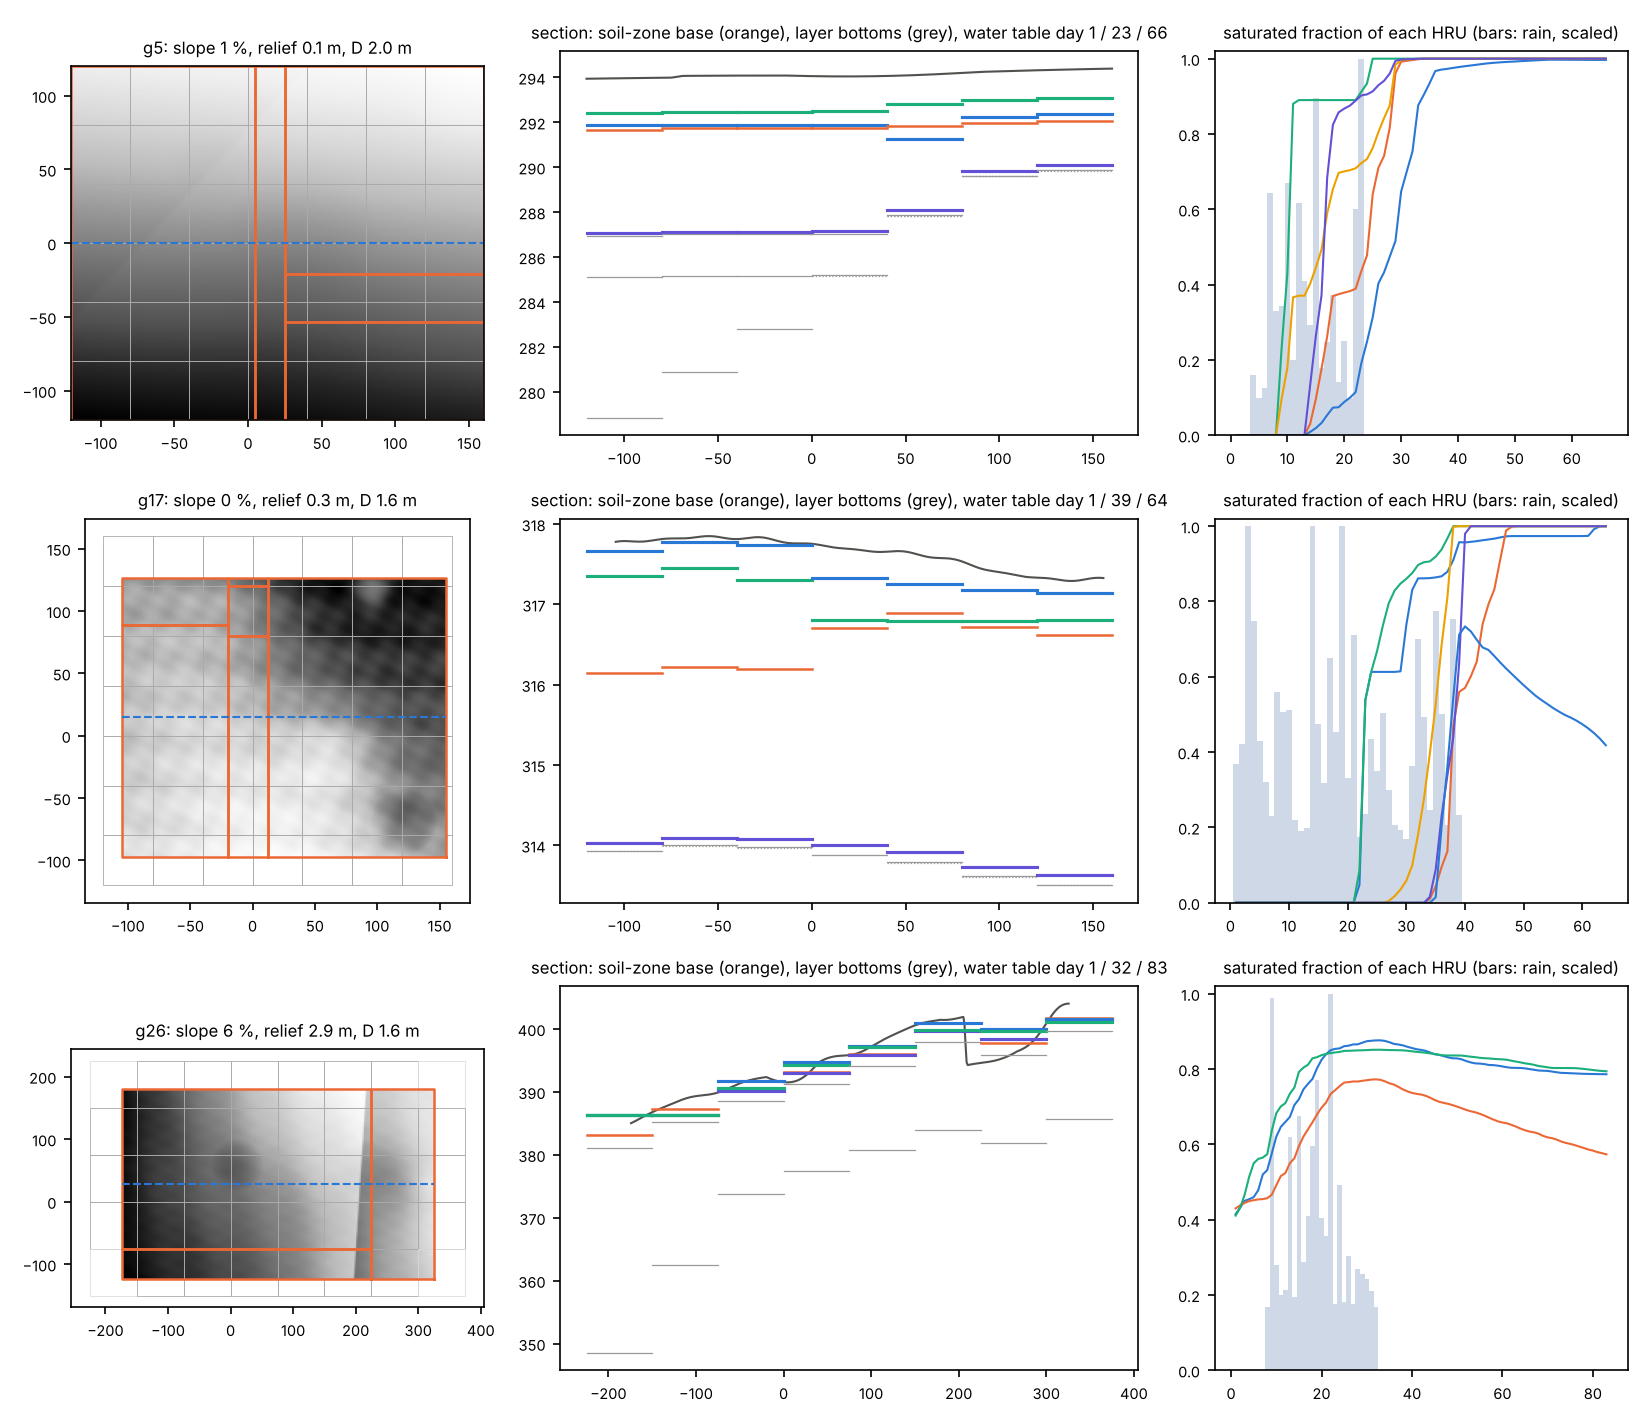
\includegraphics[width=\linewidth]{figures/fig_rough_cases.png}
\caption{Three cases of the suite (\cmd{:SoilZoneVadose NONE}). Left: DEM (shaded), grid cells and HRUs (orange); the
dashed line marks the section. Middle: land along the section, soil-zone base, MODFLOW layer bottoms of the cells it
crosses and the water table at the start, at the end of the rain and at the end of the run. Right: saturated fraction of
each HRU over the run.}\label{fig:vrough}
\end{figure}

\begin{refcard}{rough-terrain suite}
\begin{tabular}{@{}P{0.42\linewidth}P{0.53\linewidth}@{}}
\cmd{python3 test\_rough\_terrain.py} & regression cases R1--R20 and 400 seeds, \cmd{NONE} and \cmd{RICHARDS}\\
\cmd{--quick} / \cmd{--full} & 40 / 1\,500 seeds (\cmd{RAVEN\_TEST\_QUICK=1}: quick)\\
\cmd{--methods NONE,RICHARDS,KINEMATIC,LAG} & the methods run for every seed (and the regression cases whose method is listed)\\
\cmd{--vzclasses K} & \cmd{:SoilZoneVadoseClasses K} for every run\\
\cmd{--seeds a-b}, \cmd{--family gen|ext|both} & part of the seeds; generated or existing models only\\
\cmd{--case 57:RICHARDS}, \cmd{--case x43:LAG} & replay seed 57 (\cmd{x}: as an existing model); a column method is preceded by the case's \cmd{NONE} run\\
\cmd{--case rough\_cases/band\_e43.json:LAG} & replay a stored case with its own checks (or a run folder's \cmd{case.json}); the exit status is the run's\\
\cmd{--keep}, \cmd{--noreg} & keep the run folders; skip the regression cases\\
\end{tabular}
\end{refcard}
